\documentclass[twocolumn]{article}
%\usepackage{cite}
\usepackage{graphicx}
\usepackage{hyperref}
\hypersetup{colorlinks=true}

\begin{document}
\title{\vspace{-2cm}Protocol: Designing DNA-Primers for PCR}
\author{Jack Reddan}

\maketitle{}

%\tableofcontents{}

\section{Purpose}
This protocol is intended for those wanting to design DNA oligomers to be used as primers for PCR.
This protocol will not describe how to identify the sequence you wish to amplify,
since this is variable depending on what you wish to accomplish.
Therefore, a prerequisite for this protocol is to already have a target sequence in mind.

\section{Method}
\begin{enumerate}
	\item Identify the first 18--21 base pairs at the 5'-end of the sequence which has a $T_m$ within 1$^\circ$C of the preferred $T_m$.
	\item Ensure that the $\Delta G^\circ$ for this oligonucleotide's homodimer is $\ge -10$ kcal.
	\item It is preferred if the base pair at both the 5'-end and the 3'-end are G/C pairs (a G/C-cap), although, if this is not possible, then prioritize the 3'-end.
	\item Repeat steps 1--3 for the 3'-end of the sequence.
	\item Ensure that the $\Delta G^\circ$ for these oligonucleotides' heterodimer is $\ge -10$ kcal/mol.
	\item Repeat steps 1--5 for each sequence of interest.
\end{enumerate}

\section{Tips and Troubleshooting}
\begin{itemize}
	\item You can use \href{https://benchling.com/editor}{Benchling} for all $T_m$ and $\Delta G^\circ$ calculations \autoref{fig.1}.
	\begin{itemize}
			\item Concentrations can be changed by selecting the wrench next to the $T_m$ estimate under the header \textbf{Verify}.
			\item Reaction temperature can be changed next to the button `\texttt{Check Secondary Structure}' next to the header \textbf{Verify}.
	\end{itemize}
	\item The order of importance for each parameter is as follows:  $\Delta G^\circ$ (homodimerization) $\ge T_m > \Delta G^\circ$ (heterodimerization) $>$ G/C-cap $>$ length. \textbf{Only reference this hierarchy once you have tried to optimize all parameters.}
	\item Attempt to obtain a similar $T_m$ for both primers (within 0.5--1$^\circ$C).
	\item All calculations should be done before appending 5'-homology if amplicons are to be used in homology-mediated recombination (e.g., Gibson cloning).
\end{itemize}

\begin{figure}[h]
	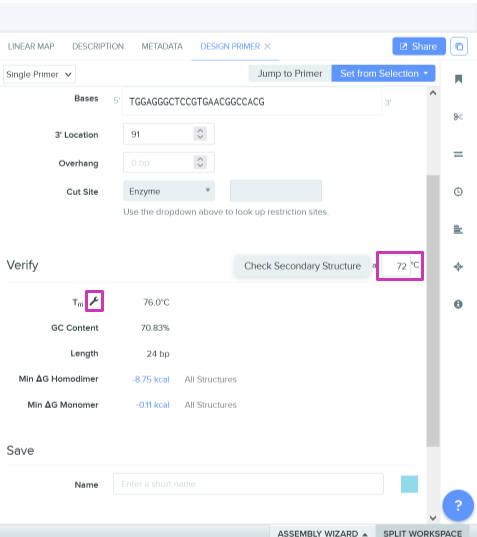
\includegraphics[width=\linewidth]{figure.png}
	\caption{Screenshot from Benchling's primer editor. To open, \textbf{Right-click} DNA selection and select \texttt{Create Primer}.}
	\label{fig.1}
\end{figure}

%\bibliography{../../library-hwa_research}
%\bibliographystyle{ieeetr}

\end{document}
